\section{Orientation}
\label{sec:warmup2}

    In this introductory practice exercise, chest X-rays were provided, and the task involved training/fine-tuning a model to determine the orientation of these X-rays.

\subsection{Dataset}
    The provided dataset consists of RGB X-ray images with 948 training samples depicting various orientations and an additional 40 samples for testing. All images are of size $128$x$128$ and are oriented either as up (0), right (1), down (2), or left (4). Due to the absence of a dedicated validation set in the given dataset, I have randomly partitioned the training samples into training and validation sets in 8:2 ratio. 
\subsection{Model Used}

    For this task, I utilized ResNet18 as the backbone model with pre-trained weights from ImageNet. Since ResNet18 was originally trained on ImageNet, its output tensor has a size of (n, 1000). However, in the given problem, we are specifically dealing with 4 classes (up, right, down, left). Therefore, I introduced a fully connected layer followed by a log-softmax layer to obtain probabilities for each class. Refer to \Cref{fig:orientation_model} for a graphical representation of the model architecture.
    
    % \begin{figure}[htbp]
    %     \centering
    %     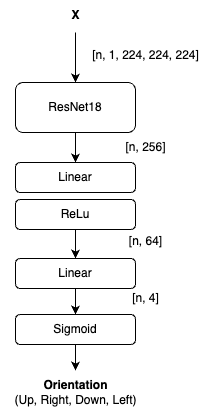
\includegraphics[width=0.4\linewidth]{images/OrientationModel.png}
    %     \caption{Graph of model used}
    %     \label{fig:model_graph}
    % \end{figure}

\subsection{Training}
    
    The model is trained using the categorical cross-entropy loss function with stochastic gradient descent as the optimizer. As the Log-Softmax layer is already included in the model, the torch.nn.NLLLoss function is employed instead of a torch.nn.CrossEntropyLoss. Four experiments were conducted with learning rates of 0.001, 0.003, 0.01, and 0.03, and the results were averaged. Refer to \Cref{fig:learning-curve} for a demonstration of the learning curve from one of the experiments.

    \begin{figure}[htbp]
        \centering
        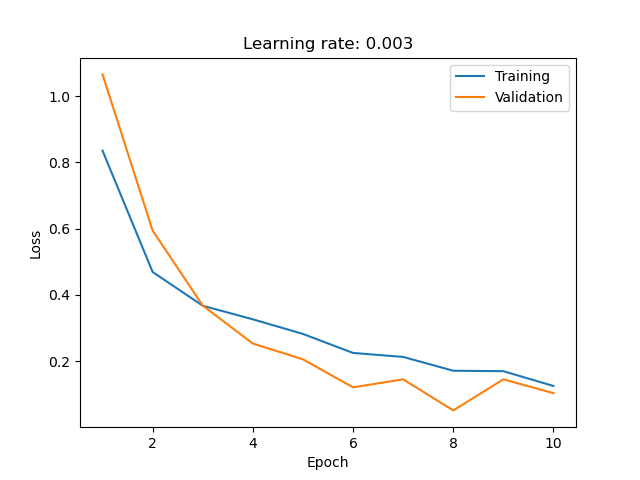
\includegraphics[width=\linewidth]{../plots/orientation/2024-01-20 21:01:42-train-val-plot.png}
        \caption{Learning curve}
        \label{fig:learning-curve}
    \end{figure}

\subsection{Results}

    \begin{figure}[!htbp]
        \centering
        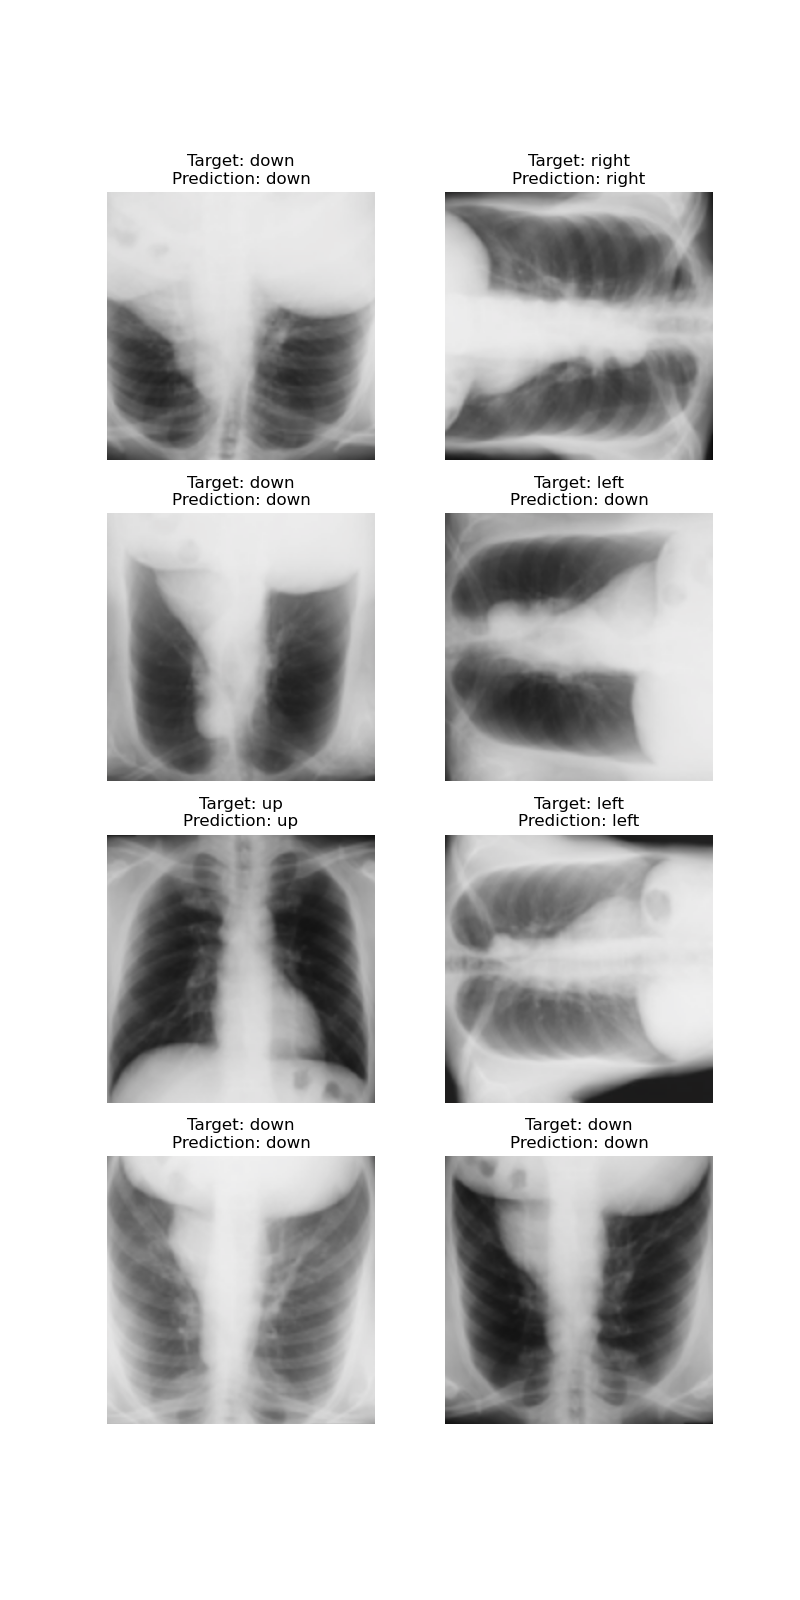
\includegraphics[width=\linewidth]{../plots/orientation/2024-01-20 21:01:42.png}
        \caption{Predictions on few samples of test data}
        \label{fig:results}
    \end{figure} 

    After fine-tuning the model with the ResNet18 backbone network, the model was transitioned to testing and evaluated on the provided test samples. On average, it achieved an accuracy of $96.87\%$, and in some experiments, $100\%$ accuracy was also attained. \Cref{fig:results} showcases some of the test samples along with their model predictions and target classes.
